\newpage
\subsubsection{W-Wing}
Die Technik \textit{W-Wing} ist die letzte und schwierigste Technik der Wings. Hierbei werden immer zwei Ziffern betrachtet. Zuerst sucht man eine Zelle, in der nur noch zwei Kandidaten x und y möglich sind. Nun wird eine Figur gesucht, in der der Kandidat x nur noch zwei mal vorkommen kann und eines der möglichen Vorkommen von der ersten Zelle ausgeschlossen würde. Im letzten Schritt sucht man eine Zelle, die wieder ausschließlich die Kandidaten x und y enthält und die das andere mögliche Vorkommen der Ziffer x in der zuvor gefundenen Figur ausschließen würde. Findet man eine solche Konstelation, dann handelt es sich um einen \textit{W-Wing}. Gelöscht werden können die  Kandidaten y, die von beiden Zellen gleichzeitig ausgeschlossen werden, da der Kandidat y entweder in der ersten oder in der zweiten gefundenen Zelle stehen muss.

\begin{figure}[h]
\begin{center}
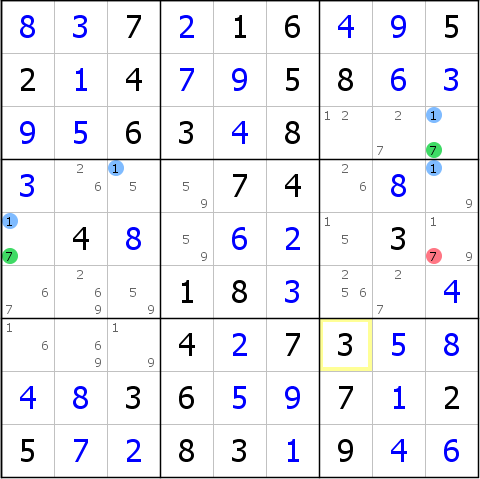
\includegraphics{./img/W_Wing.png}
\caption{W-Wing}
\end{center}
\end{figure}

\noindent In \textbf{Abbildung 2.17} betrachten wir zuerst z3s9. Hier sind die einzigen beiden Möglichkeiten 1 für x und 9 für y. Betrachten wir also zwei Fälle. Im Fall 1 nehmen wir an, dass die Ziffer 7 in z3s9 steht. Dadruch ist die rot markierte Ziffer 7 in z5s9 ausgeschlossen. Wenn die Ziffer 7 nicht in z3s9 stht, dann muss dort die Ziffer 1 stehen, das ist Fall 2. Dadurch wird die blau markierte 1 in z4s9 auschgeschlossen, was dazu führt, dass die Ziffer 1 in z4s3 stehen muss. Da dann die einzige verbleibende Möglichkeit für z4s1 die Ziffer 7 ist und diese die rot markierte Ziffer 7 in z5s9 ausschließt, kann die Ziffer 7 in z5s9 in keinem Fall dort stehen und wird gelöscht.